% \documentclass[12pt]{template}
% \begin{document}
\section{事件描述对事件参与人数的影响} 
\subsection{本章概述} 
在$\mathrm{EBSN}$中,对于一个组织者,一个非常重要的问题就是如何使自己的活动更受欢迎,借而吸引更多的人参加。而决定一件事件的属性则是相当多的,例如事件主题,举办时间,地点,所在组,事件描述等。作为这些属性中自由度最大的属性之一,问题描述在提高事件吸引力上所起的作用是显著的。例如下面两段事件描述,从直觉上来说,第一段描述显然比第二段更有吸引力。而事实也是如此,第一个事件的参与人数(超过97\%的同类事件)要远高于后者(超过5\%的同类事件)。因此,如何写出出色的事件描述,对于事件举办者而言,是个相当重要的技巧。
 
\begin{quotation}
  let  \' s get ready to get in our bikinis and board shorts  (  spe
  edos for the europeans  )  and enjoy the la summer heat on the beach
  !  this year the event is on saturday  ,  august 10th starting at 
  1pm . we will have muchies  ,  drinks and games . for those that 
  are into volleyball  ,  let  \' s repeat what we did last year . 
  i saw a lot of losers  ,  i mean winners. lol . let  \' s enjoy 
  a few good volleyball game .
    
  open to the public for a group class package and individual classes
\end{quotation}

但是想要去定量研究事件描述对事件参与度的影响,又是很困难的。一方面是因为事件描述是自然语言,难以建模,虽然近年出现的一些文本建模的方法,例如RNNLM模型,较好的克服了传统的自然语言处理中的一些问题(例如反义词),并在机器翻译,文本生成等领域取得了不错的效果,但它并不能很好的解决语义一致性的问题,例如在文本空间中,\textit{this flower smells pretty} 和 \textit{this flower smells pretty bad}会比较接近,但它们的意思是截然不同的。另外,这些方法的本质还是去拟合文本序列的概率分布,以最大化某个目标函数的期望或概率,因此很难说它们是真正理解了语义。这两方面使想要定量研究事件描述的作用变得格外困难。

在这一章中,为了解决以上问题,本文提出了事件相似度的定义,并使用了解释性较强的拉索回归对文本进行分析。提出事件相似度是因为事件的复杂性使本文必须采用合适的手段来对事件进行分类并分别度量。例如无论事件描述的好坏,一场讲座的参与人数总会比一次小型聚会来的多。所以简单的使用同一度量手段将以上两种事件一起衡量是不准确也不公平的。而这里不使用更为复杂的模型例如时序网络的原因则是受\citep{noauthor_predicting_nodate}启发,本文想观察是描述中的哪些成分对参与度有影响。比如同为聚会,包含drink的聚会是否会比包含church的聚会有更多的参与人数,而这方面的信息是可以从拉索回归中的系数获得的。由此便可以获得事件描述中的每一个词对事件结果的影响程度。

本章接下来的结构如下:在第二节,本文会定义问题,第三节会介绍事件相似度的定义,第四节则会研究事件描述对预测事件结果的影响,第五节会用来衡量事件描述中特定词语对事件结果的作用。

\subsection{问题定义}
\subsubsection{一些基本概念}
meetup\footnote{http://www.meetup.com/about},和豆瓣小组类似,是一家提供在线组织活动的平台。meetup中有三个基本对象:用户,小组,事件。具有相同兴趣的用户聚在一起组成小组,而用户也可以在小组中发布事件。用户通过RSVP来回复是否参与该事件。有些小组内的事件仅开放给组员参加,有些则对公众开放。为了方便描述,在真正的问题定义开始之前,本文先对meetup中的基本对象及其属性的表述方式作如下约定:本文使用一个七元组来表示meetup中的一个事件\(e_{id}(id,t,d,h,a,l,c)\),其中\(t\)是事件举办时间,\(d\)是事件描述,\(h\)是事件所在组,\(a\)是事件参与人,\(l\)是事件所在地点。\(c\)是事件主题:meetup的事件有36个主题。以及三元组来表示组\(g_{id}(id,e,m,c)\),其中\(e\)是事件,\(m\)是组内成员,\(c\)是该组的主题。注意到这里并没有关注成员和组的兴趣标签,虽然它在事件安排和事件推荐中的作用非常大,但在本文所研究的问题中不是值得注意的信息。

在解释了上述对象和属性后,本文就可以给该问题完整的下一个问题定义了。

\textbf{定义一: 成功事件}指对于一个事件\(e_{id}\)和与其相似的事件\(E\{e_1,e_2,e_3,...\}\),
\(|e_{id}^a|\)大于\(E\)中\(70\)\%的事件,其中$|e_{id}^a|$指事件$e_{id}$的参与人数。

衡量事件举办结果的因素有很多,这里之所以采用参与人数是因为本文想要研究的是事件参与度,而参与人数相较于其他属性则是比较直观的数值,借助于此我们可以准确的衡量一个事件在事件参与度上的表现。而且对于绝大多数事件举办者来说,如果事件参与人数超过了同类事件的百分之七十,那么该事件可以算得上是成功事件了。

\textbf{定义二: 相同事件}指对于事件\(e_{id_1}\)和事件\(e_{id_2}\),\(e_{id_1}^d=e_{id_2}^d\),其中$e_{id_i}^d$指事件$e_{id_i}$的事件描述。

在meetup中有大约30\%的事件属于相同事件,它们对于推荐算法意义重大,但如果只为了考察事件描述对事件成功的影响,则会起到相反的作用。因为在衡量事件描述产生的影响时,该类事件会增加其事件描述的影响比重,进而导致结果偏向于重复出现的事件描述。其二是参与这类事件的人有着很大的重叠,他们是基于经历而不是基于事件描述来选择参与该事件的,所以他们对事件描述不敏感。因此剔除该类事件是有必要的。对于相同事件,本文只保留其平均值。

\textbf{定义三: 相似事件}
指对于事件\(e_{id_1}\)和事件\(e_{id_2}\),\(sim(e_{id_1},e_{id_2})>\gamma\),其中\(sim\)是相似矩阵,\(\gamma\)是阈值。关于相似矩阵建立和阈值的选择可以在第\ref{s1-4}节看到。

根据以上的三个定义,最终的问题定义如下:
\newline

\textbf{定义四: 问题定义}

给定事件\(e_{id}\)和相似事件\(E\{e_1,e_2,...\}\),判断\(|e_{id}^a|\)
是否超过了\(E\)中70\%的事件。由此可见,本文把该问题转化成了一个预测问题:预测某个事件的参与人数是否超过百分之70的相似事件。
\subsection{事件相似度}\label{s1-4}
在衡量事件结果的时候,采用对所有种类的事件一视同仁的方式,使用统一的标准进行事件结果标注是不公平的。因为事件的参与人数会受到其种类的影响。如果采用统一的标准,那某些种类的事件的成功几率将会大大超过别的事件,这显然不是本文期望的。所以我们需要找到一种方式来定义事件间的相似度,让比较仅在相似度大于某一阈值的事件间发生,从而得到事件结果的标注。

由meetup上的数据来看,一个事件由时间,地点,主题,举办者,举办组等属性决定,因此,可以通过定义这些属性的相似度来定义事件的相似度。本文在定义相似矩阵的时候,主要依据的是人的主观想法:两个事件,如果主题相似,距离相近,时间相近,所在组相似(相同),那么它们很有可能是相似的。相应的,本文希望能借助相似矩阵来排除掉百分之80以上的其他事件,这可以通过调整参数来得到。

接下来,本文将分别定义举办组的相似度,事件主题相似度,时间相似度和地点相似度,从而引出地点相似度。
\paragraph{举办组的相似度}
两个组的相似可以分为两个方面,一是组的主题相似,二是组的成员相似。分别的,本文对应定义了两个矩阵:

\textbf{(a) 主题相似度} \(group\_cat\_sim:\)

\begin{equation}
group\_cat\_sim(i,j)=\frac{|g_i^c\bigcap g_j^c|}{|g_i^c|}
\end{equation}


\textbf{(b) 成员相似度} \(group\_mem\_sim:\)

\begin{equation}
group\_mem\_sim(i,j)=\frac{|g_i^m\bigcap g_j^m|}{|g_i^m|}
\end{equation}

其中$g_i^c$为组$g_i$的所有类别标签集合,$g_i^m$为组$g_i$的成员集合,通过这两个矩阵的线性组合,我们就能衡量出两个组间的相似度。

\paragraph{事件主题相似度}

和组主题相似度类似,定义如下:

\begin{equation}
event\_cat\_sim(i,j)=\frac{|e_i^c\bigcap e_j^c|}{|e_i^c|}
\end{equation}

其中$e_i^c$为事件$e_i$的所有类别标签集合。
\paragraph{时间相似度}

本文希望相似的事件在时间上也更接近,时间相似度越大。同时本文也希望确保时间相似度的值域能在\([0,1)\)之间,因此,使用负指数函数。

\begin{equation}   
time\_sim(i,j)=\mathrm{e}^\frac{-|e_i^t-e_j^t|}{\lambda}
\end{equation}

其中$e_i^t$为事件$e_i$的举办时间,\(\lambda\)为预先设置的参数。

\paragraph{地点相似度}

同样的,距离越近的事件地点相似度越高。这里使用haversine公式计算出两点之间的距离

\begin{equation}   
loc\_sim(i,j)=\mathrm{e}^\frac{-|e_i^l-e_j^l|}{\eta}
\end{equation}
其中$e_i^l$为事件$e_i$的举办地点的坐标,$\eta$为预先设置的参数。
\paragraph{事件相似度}
基于以上5个矩阵,本文所定义如下事件相似矩阵:

\begin{multline}   
event\_sim(i,j)=\alpha*group\_mem\_sim+\beta*group\_cat\_sim
\\+{c}*time\_sim+{d}*loc\_sim+{e}*event\_cat\_sim
\end{multline}

其中\(\{\alpha,\beta,{c},{d},{e}\}\)都是归一化后的参数,至于阈值\(\gamma\)的选择则应该参考\(event\_sim\)的值的分布,在实验中本文使用了前20\%的数值。

\subsection{处理事件描述}
在处理事件描述上,本文有两个选择:一是将其中出现的每一个词都视作一个事件的属性,该属性的值为此事件的事件描述中出现该词的次数。另外一个选择是先使用某种方式对事件描述进行预处理,然后将预处理后得到的对应值作为事件描述的属性值,这里不妨将预处理后得到的值称为事件描述的\textbf{评价},将对应的预处理方式称为\textbf{事件描述评价器}。如果采用了第一种方法,由于将每一个词都看作事件的一个属性,事件的特征向量的维度会变得很高(事件描述的词汇数加上其他事件属性),从而影响分类的结果。所以本文采用了第二种方法。

\paragraph{文本预处理}
由于爬取的数据描述为HTML格式,同时包含很多非英语词,例如表情,HTML控制标签。因此,在正式在预处理之前,本文对文本进行如下处理:1)去除所有非英文词和HTML标签。2)去除停止词。3)将数字替换为"\#",将出现次数少于5次的词替换为“<ukn>”。

\paragraph{事件描述评价器}

在设计事件描述的评价指标的时候,本文的初衷是评价越高的事件描述吸引力越大。但由于本文无法客观的衡量一段文本的吸引力。同时由于数据太多,也不可能采用人工打分的方式来标注数据。所以本文采用了更直接的方式:事件参与人数的对数值。这指标也和本文对事件结果的标注方式保持一致。

本文选择了拉索回归作为回归算法。这里使用拉索回归的方式是因为其比较简单,易于实现的特性。本文将在第四章探讨更复杂的回归算法对预测事件结果的改变。具体的模型如公式(\ref{1-1})和公式(\ref{1-2})所示。
\begin{equation}\label{1-1}
argmin\left\{\displaystyle\sum_{i=1}^N\left(y_i-\beta_0-\displaystyle\sum_j\beta_jx_{ij}\right)\right\}
\end{equation}
\begin{equation}\label{1-2}
subject\ to \displaystyle\sum_j|\beta_j|\leq\alpha_0\
\end{equation}

其中\(y_i\)为第\(i\)个目标即参与人数,\(x_{ij}\)为\(e_i^d\)中第\(j\)个单词。\(\alpha_0,\beta_0\)为预先设定的参数。在训练完成后,本文将使用它对事件描述进行回归,并使用其值代替原先的事件描述。

\subsection{衡量事件描述的重要性}\label{s1-5}
为了定量描述事件描述在预测事件结果中的重要性,本文参考了\citep{noauthor_predicting_nodate}中的方法:建立关于事件属性和事件参与人数的混合模型,通过衡量增删某一属性对事件属性的随机效应的确定系数的变化,来衡量增删的那一个属性的重要程度。

在介绍接下来的模型前,本文先简单介绍一下将要用到的线性混合模型。线性混合模型(\textit{Linear mixed model})是对线性模型的扩展。通过增加固定效应和随机效应,线性混合模型能很好的表示数据中某些非独立的属性对结果的影响。例如性别对于身高来说就是非独立的属性。而对应本文中所使用的数据,就是事件种类,举办地点等属性作为离散变量对于事件参与人数是非独立的。但是事件描述和组内人数则是相对独立的,因此在这里使用线性混合模型来描述这些属性和参与人数的关系是非常自然的一件事情。

本文使用了混合模型对参与人数与事件的属性之间的关系进行描述。注意到这里本文并不是想根据事件各个属性去推算事件参与人数,而是想衡量事件描述在整个模型中起的作用。本文建立的混合模型如下:

\begin{equation}
y_{ijkm}=\beta_0+log|g_i^m|+\gamma_j+\alpha_k+ (\phi_m) +\epsilon_{ijkm}
\end{equation}

其中\(\gamma_j\),\(\alpha_k\)和\(\phi_m\)为事件主题,事件举办人和事件描述的随机效应,固定效应为组内人数。本文使用Nakagawa和Schielzeth\citep{nakagawa_ageneralandsimplemethodforobtaining_2013}提出的确定系数\(R^2\)作为衡量随机效应和固定效应分别对模型的作用,在混合模型中,确定系数分为两种,一是\(R_m^2\),衡量固定效应对模型的作用,二是\(R_c^2\),衡量所有效应对模型的作用。计算方法如下:

\begin{equation}
R_m^2=\frac{\sigma_m^2}{\sigma_m^2+\sigma_\gamma^2+\sigma_\alpha^2+(\sigma_\phi^2)+\alpha_\epsilon^2}
\end{equation}
\begin{equation}
R_c^2=\frac{\sigma_m^2+\sigma_\gamma^2+\sigma_\alpha^2+(\sigma_\phi^2)}{\sigma_m^2+\sigma_\gamma^2+\sigma_\alpha^2+(\sigma_\phi^2)+\alpha_\epsilon^2}
\end{equation}

对应到本文建立的模型中,\(R_m^2\)衡量的是组内人数对事件参与人数的影响,而\(R_c^2\)衡量的是事件主题,事件举办人和事件描述对参与人数的影响。

\subsection{实验结果与分析}
本文将通过两个实验来分别预测事件结果和衡量事件描述对事件结果的影响。第一个实验即预测事件结果,本文将把事件描述作为一个附加属性,通过比较预测事件结果的变化,来衡量事件描述的作用:首先,使用第\ref{s1-4}节定义的\(event\_sim\)选出相似的事件。然后根据事件成功的定义,对事件进行标注,然后使用事件训练分类器,比较包含事件描述和不包含事件描述对分类结果的影响。第二个实验即衡量事件描述这一属性的重要程度:本文将建立关于参与人数的混合模型,并将事件描述作为可选项,比较包含和不包含事件描述对随机效应的确定系数的影响。

\subsubsection{数据集}
本次实验所使用的数据集为洛杉矶市近两年的部分活跃组别和其成员及事件。本文使用了meetup提供的api\footnote{https://www.meetup.com/meetup\_api}爬取了这部分数据。数据的详细信息如表\ref{t1-1}。
\begin{table}[htbp] 
  \centering  
  \caption{\label{t1-1}LA中近两年的meetup数据}
    \begin{tabular*}{\linewidth}{p{0.5\linewidth}p{0.5\linewidth}}
\toprule
    & LA \\
\midrule
    Users & 172673\\
    Events & 166829\\
    Groups & 2507\\
\bottomrule
    \end{tabular*}
\end{table}

\subsubsection{计算事件相似度}
本文根据之前第四节提出的方法计算出了\(event\_sim\)矩阵,其中\(\{\alpha,\beta,{c},{d},{e}\}\)分别为\(\{\frac{1}{8},\frac{1}{8},\frac{1}{4},\frac{1}{4},\frac{1}{4}\}\)。得到的相似矩阵的值的分布(图(\ref{f1-1}))。

\begin{figure}[htbp]
  \centering
  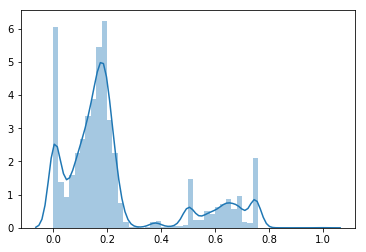
\includegraphics[width=10.4cm]{event_sim_dist.png}
  \caption{实验结果}
  \label{f1-1}
\end{figure}

可以看出相似矩阵值在0.5附近有较大的差异,并且分布比例也恰好在8:2左右,因此我们把阈值取为0.5。然后通过事件成功的定义来对所有事件的成功性进行标注。

\subsubsection{训练事件结果分类器}
为了初步的衡量事件的描述对事件参与人数的影响,可以将描述作为一个可选的属性,使用一些常用的分类器,例如随机森林,adaboast,对事件成功性进行预测。如果加入的属性提高了预测结果的准确率,那么便可推测,该属性会对事件结果产生正向的影响。在训练事件评价器时,本文从去重的原始数据中抽取了百分之50的事件,并将其移除数据库,以免对接下来的实验结果造成干扰。在正式训练分类器时,本文从数据库中抽取了10000条数据,并采用了重复采样的方式使正负数据比例达到50\%:50\%,以避免不平衡数据集对实验结果带来的影响。

最终本文使用adaboost,决策树,knn和随机森林作为分类器,使用4折交叉验证来衡量结果,使用网格搜索来确定最佳参数。本次实验平台为i5-4200m,内存为8G,显卡为gtx-730m。实验结果如表\ref{t1-3}:

\begin{table}[htbp] 
  \centering
  \caption{\label{t1-3}不同分类器下包含/不包含事件描述对预测事件结果的影响}
  \begin{tabular*}{\linewidth}{p{0.33\linewidth}p{0.33\linewidth}p{0.33\linewidth}}
\toprule 
分类器&不包含事件描述&包含事件描述\\
\midrule
Adaboost & 0.762 & 0.798 \\
决策树& 0.772 & \textbf{0.806} \\
Knn & 0.764 & 0.802  \\
随机森林 & 0.756 & 0.792 \\
\bottomrule
  \end{tabular*}
\end{table}

通过实验结果可以看出,加入了事件描述后,分类的精度有了最多百分之三的提高,间接证明了事件描述能够影响事件结果。但同时可以看出,事件描述对结果的提高是有限的。这是由于多种原因造成的:一是由于文本处理的方式过于粗糙,拉索回归仍然过于简单,它处理线性相关的数据比较有效,而文本和事件参与人数不全是线性相关的。二是由于样本太少(交叉验证时每次训练量大概只有3000条),三是由于在某些情况下事件描述对事件结果不起决定性作用。能影响事件参与人数的因素非常多,当其他因素起决定性作用的时候,事件描述的好坏就不再是那么重要的了。

\subsubsection{衡量事件描述在事件属性中的重要程度}
本文建立了\ref{s1-5}中的混合模型。我们使用了R语言中的``lme4''计算包\citep{lme4}实现上文的模型,\(R^2\)的计算使用了R语言中的``MuMIn''计算包\citep{MuMIn}。结果如表\ref{t1-4}。

\begin{table}[htbp]
  \caption{\label{t1-4}包含事件描述与否的情况下固定效应和随机效应的确定系数}
	\centering  
    \begin{tabular*}{\linewidth}{p{0.33\linewidth}p{0.33\linewidth}p{0.33\linewidth}}
  \toprule
    &  \(R_c^2\) & \(R_m^2\) \\ 
  \midrule
		包含事件描述                       & \textbf{0.653} & 0.135 \\ 
    不包事件含描述                        & 0.494 & 0.135 \\ 
  \bottomrule
    \end{tabular*}
\end{table}

可以看出包含事件描述后,\(R_c^2\)显著提高,这说明加入了事件描述后,模型的解释性得到了增强,从而证明了事件描述在事件属性中的重要性。另一个值得注意的是组的规模的确定系数只有0.135,这说明了组内人数对事件参与人数并没有特别显著的影响。

\subsection{衡量事件描述中特定词语的影响}
在上文的实验中,本文使用了拉索回归作为事件描述评价器的回归算法。同时提到了由于事件描述和事件参与结果之间不完全是线性关系,所以这里拉索回归并不是十分理想的评价模型,而在实验结果中我们也可以发现添加事件描述后最终预测事件结果的准确率的提升也不是很明显。但是,虽然事件描述和事件参与结果之间不是线性关系,但如果不考虑文本的序列性,而仅仅将文本看做词的集合,那么事件描述和事件参与结果之间就可以近似的看做线性关系了。

在这种假设下,事件描述对事件结果的影响就可以看做是每一个词的影响的依次叠加,从而便可以通过考察每个词对应的系数的大小,来定量衡量其对事件结果的影响。拉索回归在处理这种问题有着天然的优势。因为拉索回归有一个非常独特的性质,在于它的损失函数。与传统线性回归的损失函数不同的是,它的损失函数中包含了$\mathrm{L1}$正则的罚函数,导致在拉索回归中,大部分属性的系数值为零,即对结果没有影响。因此,拉索回归可以起到筛选变量的作用\citep{tibshirani_regression_1996}。所以,本文便可以由拉索回归的系数矩阵,通过比较回归系数的绝对值大小,来挑选出对参与人数影响比较大的单词。而通过比较回归系数的正负,我们便可以得知该词对事件结果起正面还是负面作用了\citep{noauthor_predicting_nodate}。

在这里本文使用了上文实验训练好的事件描述评价器中的系数矩阵,挑选出系数最高和系数最低的9个词,结果如表\ref{t1-2}通过观察结果,可以发现,在系数最高/最低的词中,有些词符合人的主观判断,例如cocktails。想必在有party文化的洛杉矶,鸡尾酒对人的吸引应该是很大的有些则不那么直观,比如spiritual。但如果找到包含这个词的事件描述,可以发现它常常出现在教堂组织的礼拜活动中,所以参与者不是那么多。

虽然某些词语可以对事件结果起正面影响,但有一点值得注意的是,作为事件组织者,如果在编写事件描述的时候,大量的使用这些正向词汇,是无法达到吸引更多的人来参加的效果。因为这样做成立的假设条件是将文本看做词的集合,但在现实生活中,这种假设显然是不成立的,而序列信息是文本非常重要的信息之一。

\begin{table}[htbp]
  \caption{\label{t1-2}对参与人数的影响比较重要的词}
    \centering
      \begin{tabular*}{\linewidth}{p{0.15\linewidth}p{0.35\linewidth}p{0.35\linewidth}p{0.15\linewidth}}
  \toprule      
      &系数最高的9个词 & 系数最低的9个词&\tabularnewline
  \midrule
  &christmas & week&\tabularnewline
  &dance & saga&\tabularnewline
  &directions & meditation&\tabularnewline
  &cocktails & information&\tabularnewline
  &concerts & salt&\tabularnewline
  &band & mammoth&\tabularnewline
  &perfect & spiritual&\tabularnewline
  &tribute & masked&\tabularnewline
  &drinks & learn&\tabularnewline
  \bottomrule
      \end{tabular*}
  \end{table}

\subsection{本章小结}
本章主要研究了事件描述对事件参与人数的影响。本文首先定义了事件相似性,以消除事件种类的差异性对标注事件结果的影响。同时使用了拉索回归的方式对事件描述进行了预处理,以抵消高维系数的属性向量对分类器的影响。然后通过对比实验,使用一系列分类器证明了事件描述可以帮助提高预测事件结果的准确率,最后为了衡量增加事件描述后对模型解释性的影响,建立了线性混合模型,并比较了增加了事件描述后事件属性的随机效应的确定系数的变化。实验证明了增加事件描述并不只是增加了多余的信息,而是提高了模型的解释能力,由此得出事件描述是影响事件是否成功的非常重要的一环的结论。最后为了衡量事件描述中的词语对事件结果的影响,比较了拉索回归后得到的系数矩阵,发现特定词对事件结果的影响基本符合人的客观认知。

然而,值得注意的是,这里本文使用的方法仍然是十分简略的,首先,在处理文本的时候将文本序列视作词的集合,这也是在本节中使用拉索回归的一个重要原因。然而,虽然最终拉索回归也能提高事件预测准确率,在衡量词对事件结果的影响时也得到了可解释的结果,但其简单的特性也导致了其会损失很多信息,例如文本中的序列信息。而这些信息对于提升对预测事件结果的准确率是十分重要的。所以接下来,本文会去尝试更复杂的模型,以探索能否在原来的基础上,进一步提高预测的准确率,甚至在不考虑其他因素的情况下,仅凭借事件描述这一属性,就预测出事件的参与度。这在现实中也是有意义的:事件组织者可以借助这种工具来预估事件参与人数,以更好的准备举办事件的前期工作。这部分工作将在第四章得到阐述。

另一个值得注意的地方是如何产生新的事件描述的工作。近年来在机器翻译,新闻自动撰写等方面的文本生成工作获得了长足的发展,借助序列到序列和对抗网络,本文可以生成通顺的,质量足够高的文本。这也给本文启示:一方面,帮助事件组织者判断他们的事件描述是否足够好是有意义的工作,但是如果能自动生成一些有意义的事件描述,也是件有趣的事情。我们将在第五章介绍这部分工作。

% \end{document}